% ============================================================
% CAPITOLO 1 — SPECIFICHE DEI REQUISITI SOFTWARE (SRS)
% ============================================================
\chapter{Specifiche dei Requisiti Software}
\label{cap:srs}

% ------------------------------------------------------------
\section{Introduzione}
\label{sec:intro}

\subsection{Scopo del documento}
\label{subsec:scopo}

Questo documento definisce i requisiti software di \textbf{CiboAmico}, il progetto finale del corso ISPW (Università di Roma ``Tor Vergata'', A.A.\ 2025/2026, Prof. Davide Falessi, Prof. Guglielmo De Angelis).

Lo scopo è fissare cosa il sistema deve fare in modo chiaro e verificabile, lasciando campo alla progettazione e ai test. Il documento serve sia a chi sviluppa, per tenere fede all'architettura Boundary-Control-Entity (BCE), sia a chi valuta il prodotto, per confrontare i flussi funzionali con le richieste iniziali.

\subsection{Panoramica del sistema}
\label{subsec:panoramica}

CiboAmico è un'applicazione desktop JavaFX che aiuta a gestire il cibo in casa, evitare sprechi e ottimizzare la spesa, collegando l'utente ai commercianti di prossimità. Il sistema segue il pattern Boundary-Control-Entity (BCE) e coinvolge quattro attori: Cliente, Venditore, Nutrizionista e Amministratore. Due sistemi esterni sono raggiunti tramite Adapter: OpenFoodFacts (lettura dei dati nutrizionali dal codice a barre) e JakartaMail (invio di notifiche). La persistenza è intercambiabile a runtime tra una modalità \textit{Demo} (in-memory) e una \textit{Full} (MySQL via JDBC).

Il sistema ha tre aree funzionali:
\begin{itemize}
    \item \textbf{Dispensa}: il Cliente traccia i prodotti in casa, vede le scadenze e viene avvisato prima che il cibo si deteriori;
    \item \textbf{Ricette}: il sistema propone ricette compatibili con gli ingredienti disponibili, sostituendo quelli mancanti;
    \item \textbf{Marketplace}: i Venditori pubblicano i prodotti, i Clienti fanno ordini diretti (un compratore, un venditore) e l'Amministratore approva venditori e ricette.
\end{itemize}

\subsection{Requisiti hardware e software}
\label{subsec:requisiti_hw_sw}

L'applicazione è cross-platform grazie alla JVM. I requisiti minimi sono: processore dual-core a 64-bit, 2~GB di RAM, 150~MB di disco e schermo $1024\times768$. In modalità JDBC, che esegue anche il server MySQL locale, si consigliano 4~GB di RAM, 500~MB su SSD e una scheda grafica compatibile con OpenGL 2.0.

A livello software servono: OpenJDK 17 LTS, JavaFX 17+, Maven 3.9+ e, per la modalità database, MySQL 8.0+. Per sviluppo e controllo qualità si usano IntelliJ IDEA (con EclEmma per la coverage), JUnit 5, SonarCloud e GitHub Actions. I diagrammi UML sono realizzati con StarUML o Draw.io.

\subsection{Sistemi correlati, pro e contro}
\label{subsec:relazionati}

Di seguito due sistemi esistenti che coprono solo in parte quello che fa CiboAmico.

\paragraph{Too Good To Go}
Piattaforma B2C per il recupero delle eccedenze alimentari: connette l'utente con commercianti e supermercati locali.
\begin{itemize}
    \item \textbf{Pro}: rete capillare di partner con offerte geolocalizzate in tempo reale; riduce attivamente lo spreco commerciale offrendo cibo a prezzi ridotti.
    \item \textbf{Contro}: non traccia la dispensa di casa, quindi dopo l'acquisto non aiuta a gestire le scadenze; l'acquisto è una \emph{Magic Box} a sorpresa, non si scelgono i singoli prodotti né si pianificano ricette o diete.
\end{itemize}

\paragraph{SuperCook}
Motore di ricerca di ricette in base agli ingredienti già in dispensa.
\begin{itemize}
    \item \textbf{Pro}: matching potente che trova subito molte ricette a partire dagli ingredienti inseriti; ampio database con filtri per tipo di piatto e intolleranze.
    \item \textbf{Contro}: non ha un canale di acquisto integrato, quindi per gli ingredienti mancanti bisogna provvedere da soli; non sostituisce automaticamente gli ingredienti, escludendo ricette realizzabili con piccole variazioni.
\end{itemize}

\paragraph{Posizionamento di CiboAmico}
CiboAmico unisce i due approcci: gestisce la dispensa contro lo spreco (come SuperCook), propone ricette con sostituzioni intelligenti e, se manca qualcosa, permette di comprarlo dai produttori locali a chilometro zero (come Too Good To Go), tutto in una sola applicazione.

% ------------------------------------------------------------
\section{User Stories}
\label{sec:user_stories}

\begin{enumerate}
    \item \textbf{US-1}: Come Cliente, voglio ricevere notifiche preventive sulle date di scadenza dei prodotti presenti nella mia dispensa, in modo che possa consumare gli alimenti in tempo ed evitare lo spreco di cibo.
    \item \textbf{US-2}: Come Cliente, voglio visualizzare le ricette compatibili con gli ingredienti disponibili in dispensa, in modo che possa cucinare senza dover effettuare nuovi acquisti.
    \item \textbf{US-3}: Come Cliente, voglio ordinare un prodotto direttamente da un venditore locale, in modo che possa ricevere cibo fresco proveniente dal mio territorio.
\end{enumerate}

% ------------------------------------------------------------
\section{Requisiti Funzionali}
\label{sec:requisiti_funzionali}

\begin{enumerate}
    \item \textbf{RF-1}: Il sistema deve confrontare quotidianamente le date di scadenza degli alimenti nella dispensa con la data corrente, inviando un avviso al cliente per ogni prodotto la cui scadenza sia entro tre giorni.
    \item \textbf{RF-2}: Il sistema deve suggerire al cliente un elenco di ricette in cui gli ingredienti richiesti siano un sottoinsieme degli ingredienti non scaduti presenti nella dispensa.
    \item \textbf{RF-3}: Il sistema deve registrare una nuova transazione di acquisto associando il cliente al venditore e decrementando la scorta del prodotto in misura pari alla quantità ordinata.
\end{enumerate}

\subsection{Glossario dei Termini di Dominio}
\begin{description}
    \item[\textbf{Dispensa}]: rappresentazione digitale degli alimenti presenti nell'inventario domestico dell'utente, con quantità e date di scadenza.
    \item[\textbf{Ricetta compatibile}]: ricetta i cui ingredienti richiesti sono presenti, oppure sostituibili in modo equivalente, nella dispensa dell'utente.
    \item[\textbf{Ordine diretto}]: transazione che associa un singolo cliente acquirente a un unico venditore, senza passare da un carrello condiviso o intermediari.
    \item[\textbf{Disponibilità del prodotto}]: quantità di un prodotto attualmente vendibile, che non può mai essere negativa e viene aggiornata dopo ogni acquisto.
\end{description}

% ------------------------------------------------------------
\section{Use Cases}
\label{sec:use_cases}

\subsection{Diagramma dei casi d'uso}
\label{subsec:uc_diagramma}

\begin{figure}[H]
    \centering
    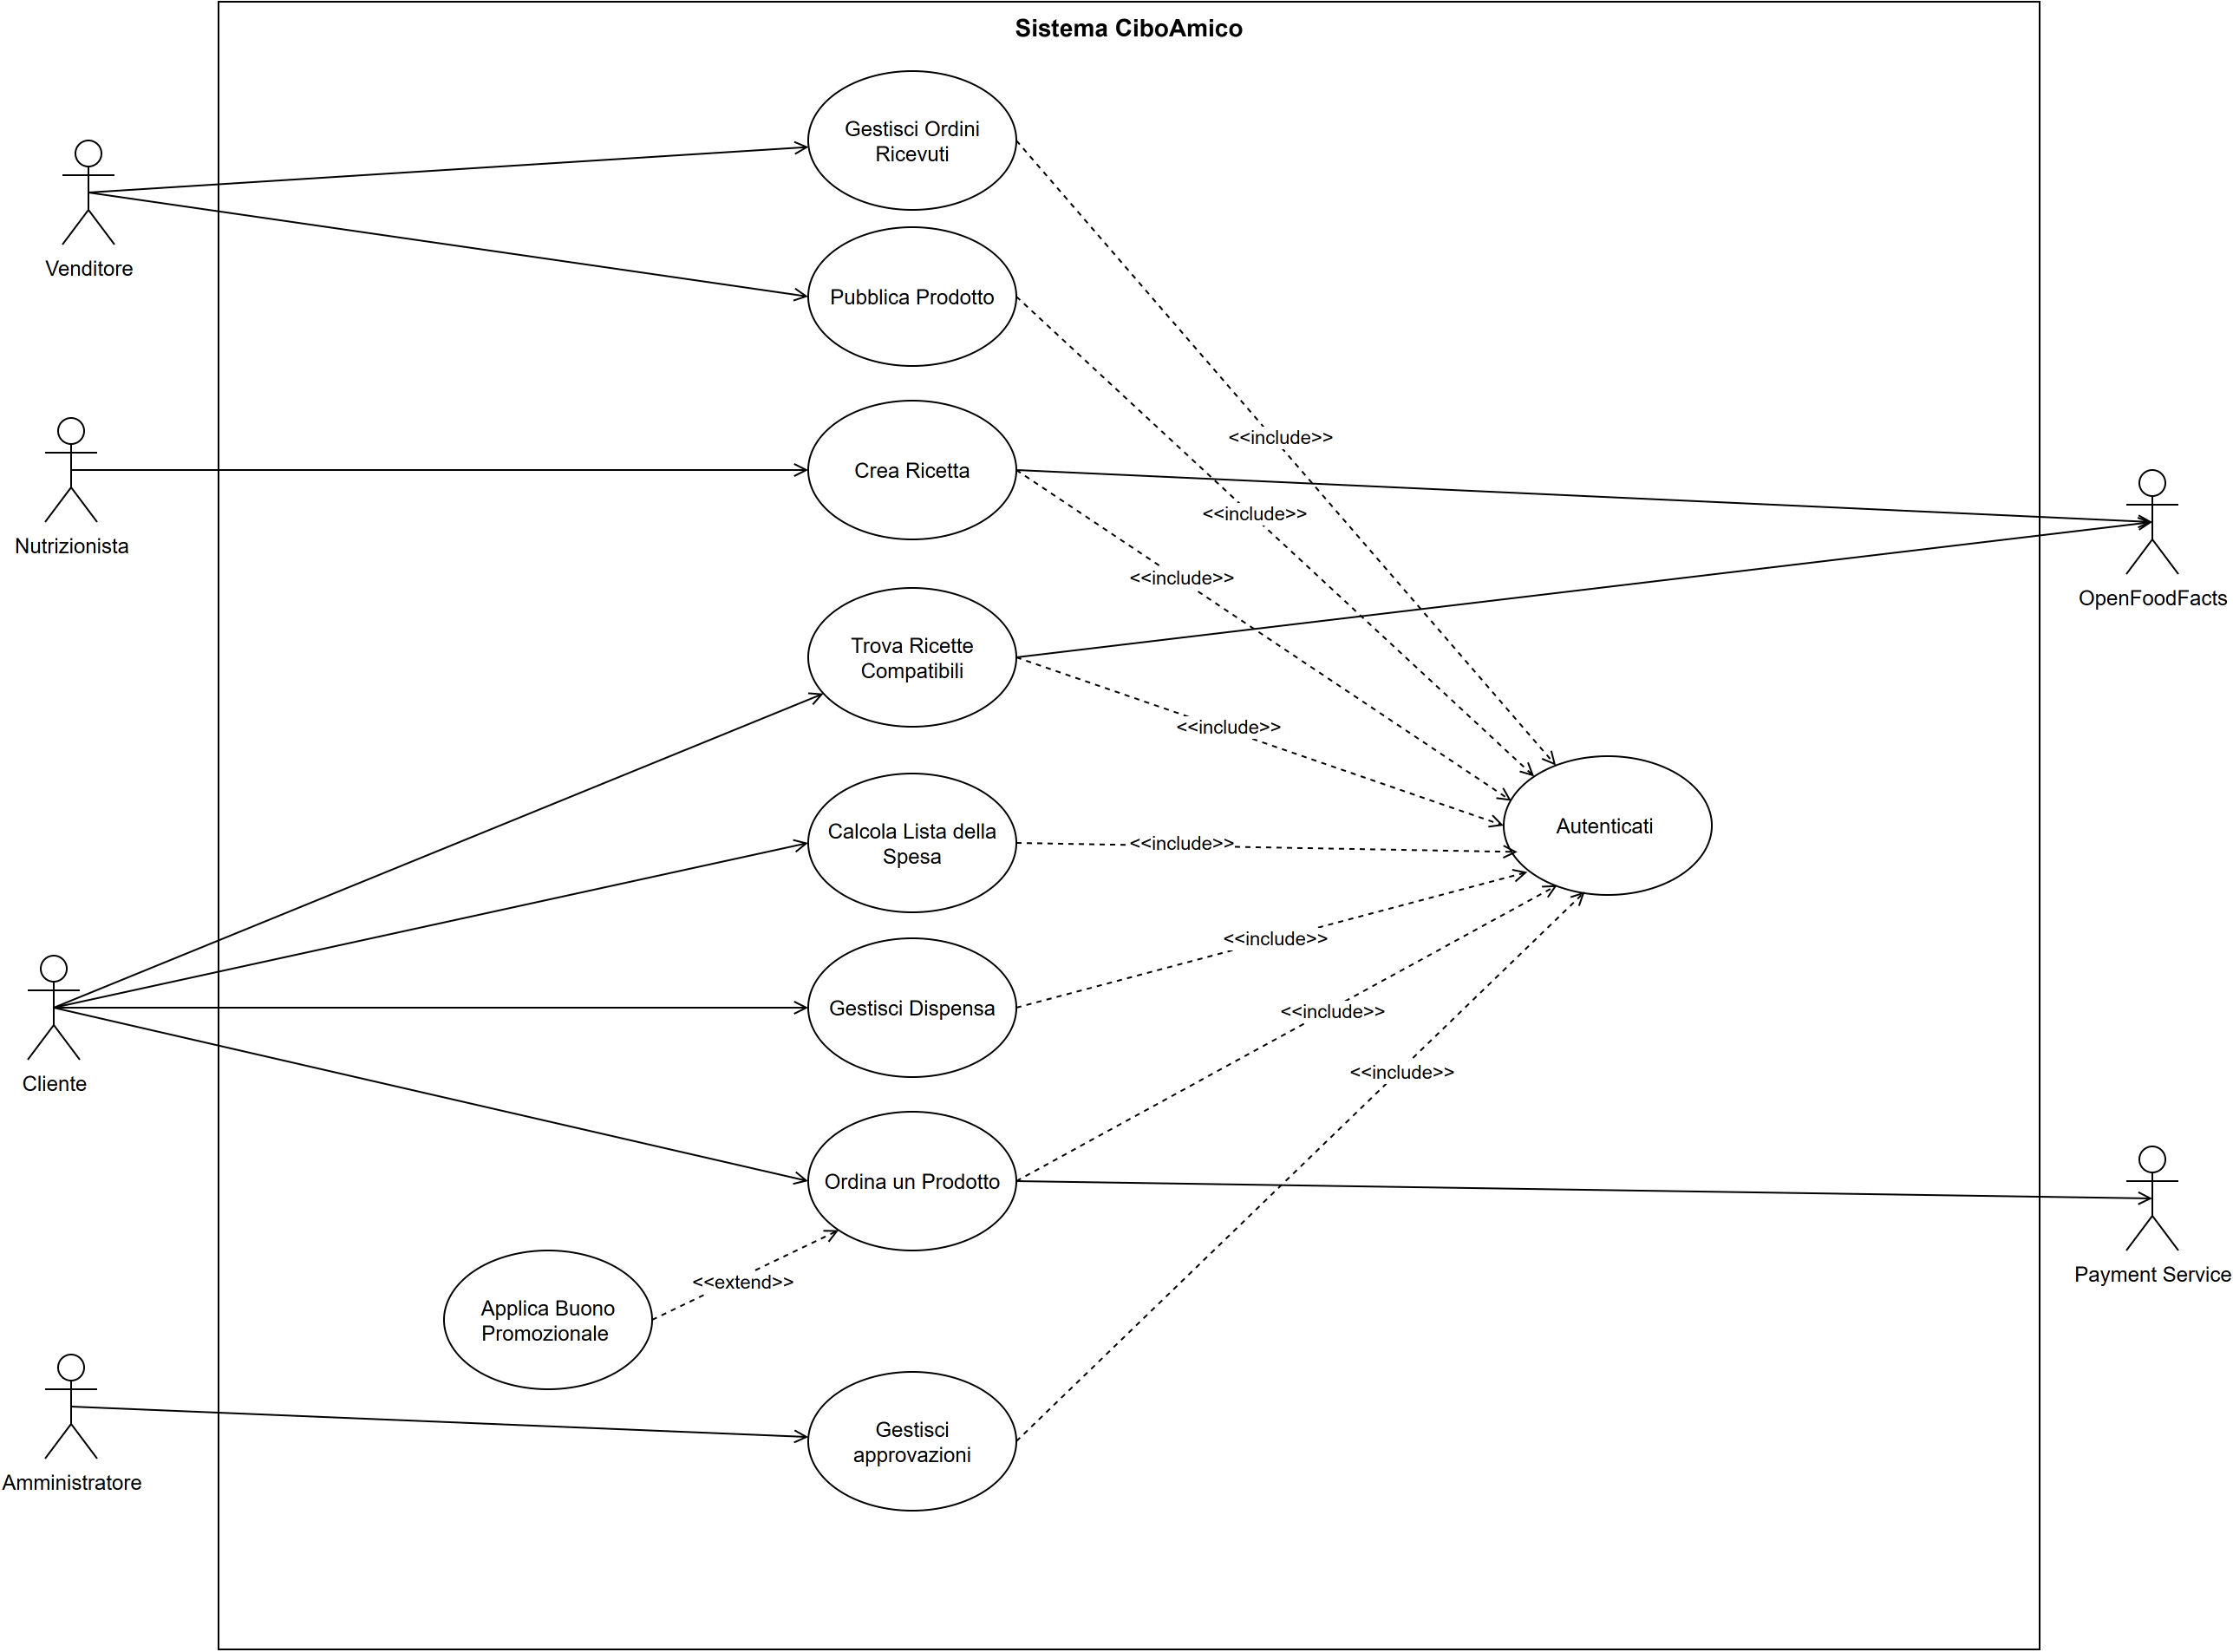
\includegraphics[width=0.95\textwidth]{figures/usecase_diagram_hr.png}
    \label{fig:usecase_diagram}
\end{figure}

Il caso d'uso \textbf{Ordina un Prodotto} è stato progettato con un grado di astrazione che consente di modellare funzionalità distinte. In questa implementazione, il caso d'uso secondario \textbf{Applica Buono Promozionale} è associato al caso d'uso primario tramite una relazione di \emph{extend}: l'attore Cliente può utilizzare questa funzionalità estesa solo se si autentica correttamente nel sistema (relazione di \emph{include} verso \textbf{Autenticati}) e proseguendo poi il flusso del caso d'uso \textbf{Ordina un Prodotto}. Analogamente, \textbf{Autenticati} è incluso da più casi d'uso, a sottolinearne il riuso nell'ambito delle funzionalità principali.

\subsection{Internal Steps}
\label{subsec:uc_internal_steps}

\subsubsection{Ordina un Prodotto}
\label{u:uc04}

\textbf{Scenario principale:}
\begin{enumerate}
    \item Il Sistema individua i prodotti disponibili sul marketplace con prezzi, scorte residue e venditori.
    \item Il Cliente richiede di aggiungere un prodotto all'ordine, indicandone la quantità desiderata.
    \item Il Sistema convalida che la quantità richiesta non superi la scorta residua del prodotto.
    \item Il Sistema calcola l'importo totale della transazione. \label{step:calcolo_totale}
    \item Il Cliente richiede di confermare l'acquisto. \label{step:conferma_acquisto}
    \item Il Sistema richiede al Payment Service l'autorizzazione all'addebito per l'importo calcolato.
    \item Il Sistema registra l'ordine in attesa di approvazione e decrementa la scorta residua dei prodotti ordinati.
    \item Il Sistema invia una notifica al Venditore per segnalare l'ordine ricevuto.
\end{enumerate}

\textbf{Estensioni:}
\begin{itemize}
    \item \textbf{3a. Superamento della scorta residua:}
    \begin{enumerate}
        \item Il Sistema rileva che la quantità inserita dal Cliente è superiore alla disponibilità corrente del prodotto.
        \item Il Sistema segnala l'anomalia al Cliente indicando la massima quantità acquistabile.
        \item Il flusso di controllo ritorna al passo 2.
    \end{enumerate}
    \item \textbf{4a. Richiesta di applicazione di un buono promozionale (tramite l'estensione del caso d'uso Applica Buono Promozionale):}
    \begin{enumerate}
        \item Il Cliente richiede di applicare un codice di buono promozionale all'ordine corrente.
        \item Il Sistema convalida la validità temporale del buono promozionale e la sua associazione con il Venditore del prodotto selezionato.
        \item Il Sistema ricalcola l'importo totale della transazione applicando lo sconto previsto dal buono promozionale.
        \item Il flusso di controllo prosegue dal passo 5 dello scenario principale.
    \end{enumerate}
    \item \textbf{6a. Autorizzazione di pagamento negata:}
    \begin{enumerate}
        \item Il Sistema riceve l'esito negativo dall'autorizzazione del Payment Service.
        \item Il Sistema segnala al Cliente il fallimento del pagamento.
        \item Il flusso di controllo ritorna al passo 5.
    \end{enumerate}
\end{itemize}

